\documentclass[
  captions=tableheading,
  bibliography=totoc, 
  titepage=firstiscover,
]{scrartcl}

\usepackage{blindtext} %neuer input

\usepackage{longtable} % Tabellen über mehrere Seiten

\usepackage[utf8]{inputenc} %neuer input

\usepackage{scrhack}

\usepackage[aux]{rerunfilecheck} %Warnung falls nochmal kompiliert werden muss

\usepackage{fontspec} %Fonteinstellungen

\recalctypearea{}

\usepackage[main=ngerman]{babel} %deutsche Spracheinstellung

\usepackage{ragged2e} %neuer input

\usepackage{amsmath, nccmath}

\usepackage{amssymb} %viele mathe Symbole

\usepackage{mathtools} %Erweiterungen für amsmath


\DeclarePairedDelimiter{\abs}{\lvert}{\rvert}
\DeclarePairedDelimiter{\norm}{\lVert}{\rVert}

\DeclarePairedDelimiter{\bra}{\langle}{\rvert}
\DeclarePairedDelimiter{\ket}{\lvert}{\rangle}

\DeclarePairedDelimiterX{\braket}[2]{\langle}{\rangle}{
#1 \delimsize| #2
}

\NewDocumentCommand \dif {m}
{
\mathinner{\symup{d} #1}
}


\usepackage[
  math-style=ISO,
  bold-style=ISO,
  sans-style=italic,
  nabla=upright,
  partial=upright,
  warnings-off={
    mathtools-colon,
    mathtools-overbracket,
  },
]{unicode-math}

\setmathfont{Latin Modern Math}
\setmathfont{XITS Math}[range={scr, bfscr}]
\setmathfont{XITS Math}[range={cal, bfcal}, StylisticSet=1]


\usepackage[
  locale=DE,
  separate-uncertainty=true,
  per-mode=reciprocal,
  output-decimal-marker={,},
]{siunitx}

\usepackage[autostyle]{csquotes} %richtige Anführungszeichen

\usepackage{xfrac}

\usepackage{float}

\floatplacement{figure}{htbp}

\floatplacement{table}{htbp}

\usepackage[ %floats innerhalb einer section halten
  section,   %floats innerhalb er section halten
  below,     %unterhalb der Section aber auf der selben Seite ist ok
]{placeins}

\usepackage[
  labelfont=bf,
  font=small,
  width=0.9\textwidth,
]{caption}

\usepackage{subcaption} %subfigure, subtable, subref

\usepackage{graphicx}

\usepackage{grffile}

\usepackage{booktabs}

\usepackage{microtype} %Verbesserungen am Schriftbild

\usepackage[
backend=biber,
]{biblatex}

\addbibresource{../lit.bib}

\usepackage[ %Hyperlinks im Dokument
  german,
  unicode,
  pdfusetitle,
  pdfcreator={},
  pdfproducer={},
]{hyperref}

\usepackage{bookmark}

\usepackage[shortcuts]{extdash}

%\usepackage{warpcol}


\begin{document}
    \title{V311 Der Hall-Effekt}
    \author{  
    Tobias Rücker\\
    \texorpdfstring{\href{mailto:tobias.ruecker@tu-dortmund.de}{tobias.ruecker@tu-dortmund.de}
    \and}{,} 
    Paul Störbrock\\
    \texorpdfstring{\href{mailto:paul.stoerbrock@tu-dortmund.de}{paul.stoerbrock@tu-dortmund.de}}{}
    }
    \date{Durchführung: 21.01.20, Abgabe: 28.01.20 \vspace{-4ex}}
\maketitle
\center{\Large Versuchsgruppe: \textbf{42}}
\thispagestyle{empty}

\newpage
\tableofcontents
\thispagestyle{empty}
\newpage

% Ziel %%%%%%%%%%%%%%%%%%%%%%%%%%%%%%%%%%%%%%%%%%%%%%%%%%%%%%%%%%%%%%%%%%%%%%%%%%%%%%%%%%%%%%%%%%%%%%%%%%%%%%%%%%%%%%%%%%%%%%%%%%%%%%%%%%%%%%%%%%%%%%%%%%%%%%%%%%%%%%%%%%%%%%%%%%%%%%%%%%%%%%%%%%%%%%%%%%%%%%%%%%%%%%%%%

\setcounter{page}{1}
\section{Ziel}\justifying

% Theorie %%%%%%%%%%%%%%%%%%%%%%%%%%%%%%%%%%%%%%%%%%%%%%%%%%%%%%%%%%%%%%%%%%%%%%%%%%%%%%%%%%%%%%%%%%%%%%%%%%%%%%%%%%%%%%%%%%%%%%%%%%%%%%%%%%%%%%%%%%%%%%%%%%%%%%%%%%%%%%%%%%%%%%%%%%%%%%%%%%%%%%%%%%%%%%%%%%

\section{Theorie}\justifying

% Fehlerrechnung %%%%%%%%%%%%%%%%%%%%%%%%%%%%%%%%%%%%%%%%%%%%%%%%%%%%%%%%%%%%%%%%%%%%%%%%%%%%%%%%%%%%%%%%%%%%%%%%%%%%%%%%%%%%%%%%%%%%%%%%%%%%%%%%%%%%%%%%%%%%%%%%%%%%%%%%%%%%%%%%%%%%%%%%%%%%%%%%%%%%%%%%%%%%%%%%%%%%%%

\section{Fehlerrechnung}\justifying

Für die Berechnung von Messunsicherheiten werden in diesem Protokoll folgende Formeln
verwendet:
\begin{subequations} \label{eq:}
\begin{align} 
\intertext{Zur Bestimmung eines Mittelwertes wird folgende Formel benutzt:
}
    \overline{x} &= \frac{1}{N}\sum_{i=1}^{N} x_i \label{eq:a}
\intertext{Zur Bestimmung der Messunsicherheit bei Mittelwerten wird mit der Formel
}
    \Delta\overline{x} &= \frac{1}{\sqrt{N}} \sqrt{\frac{1}{1-N} \sum_{i=1}^{N} (x_i - \overline{x})^2} \label{eq:b},
\intertext{gearbeitet und die Gaußsche Fehlerfortpflanzung wird mit
}
    \Delta f &= \sqrt{\sum_{i=1}^{N} \left( \frac{\delta f}{\delta x_i} \right)^2 \cdot (\Delta x_i)^2} \label{eq:c}
\intertext{berechnet. Um Ausgleichsgeraden und ihre Parameter zu bestimmen, werden folgende Formeln verwendet:
}
    y &= m \cdot x + b \label{eq:6d} \\ 
    m &= \frac{\overline{xy} - \overline{x} \cdot \overline{y}}{\overline{x^2} - {\overline{x}}^2} \label{eq:e}\\
    b &= \frac{\overline{y} \cdot \overline{x^2} - \overline{xy} \cdot \overline{x}}{\overline{x^2} - {\overline{x}}^2} \label{eq:f}
\end{align}
\end{subequations}
\newpage

% Versuchsaufbau + Versuchsdurchführung %%%%%%%%%%%%%%%%%%%%%%%%%%%%%%%%%%%%%%%%%%%%%%%%%%%%%%%%%%%%%%%%%%%%%%%%%%%%%%%%%%%%%%%%%%%%%%%%%%%%%%%%%%%%%%%%%%%%%%%%%%%%%%%%%%%%%%%%%%%%%%%%%%%%%%%%%%%%%%%%%%%%%%%%%%%%%%%%%%%%%%%%%%%%%%%%%%

\section{Versuchsaufbau und Versuchsdurchführung}\justifying
Benötigt werden: \textit{Ein Eisenjoch, zwei Spulen, zwei Magnetschuhe, drei Leiterplatten, drei Materialproben (hier Cu, Zn und Ag), 
ein digitales Multimeter, zwei Generatoren (max. $\SI{40}{\volt}/\SI{10}{\ampere}$ und max. $\SI{20}{\volt}/\SI{5}{\ampere}$), 
eine Hall-Sonde, eine digitale Mikrometerschraube, einen Kupferwiderstand (Drahtlänge: $\SI{137}{\centi\meter}$, Drahtdurchmesser: 
$\SI{0.1}{\milli\meter}$), einen Silberwiderstand (Drahtlänge: $\SI{173}{\centi\meter}$, Drahtdurchmesser: $\SI{0.205}{\milli\meter}$) 
und sieben Experimentierkabel.}

\flushleft{Zu\;}\justifying Beginn wird das Eisenjoch durch beide Spulen geführt. An beiden Enden des Eisenjochs werden nun die Magnetschuhe
angebracht. Sobald der Elektromagnet aufgebaut ist, werden die beiden Spulen in Reihe geschaltet und an den Generator mit maximal 
$\SI{5}{\ampere}$ angeschlossen. Mit diesem Aufbau und der Hall-Sonde wird die Hysterese des Magnetfelds bestimmt. Dafür wird der Strom sukzessiv 
um $\SI{0.5}{\ampere}$ erhöht, bis $\SI{5}{\ampere}$ an den Spulen anliegen. Für jede Erhöhung des Stroms um $\SI{0.5}{\ampere}$ wird die Stärke
des Magnetfelds mit der Hall-Sonde abgelesen. Sind die $\SI{5}{\ampere}$ erreicht, wird der selbe Prozess wiederholt während der Strom in reduziert
wird. 

\flushleft{Sind\;}\justifying die Messwerte der Hysterese bestimmt, wird die Hall-Sonde entfernt und die erste Materialprobe auf der Leiterplatte
zwischen den Magnetschuhen befestigt. Anschließend wird die Leiterplatte wie folgt an dem Multimeter angeschlossen:

\begin{figure}
    \centering
    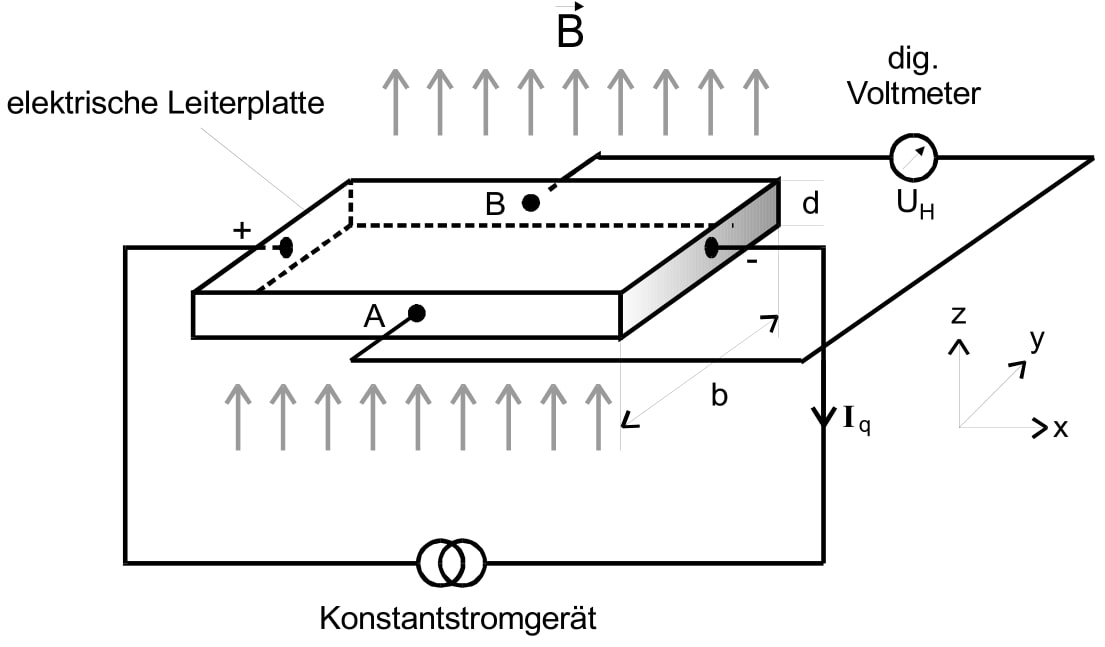
\includegraphics[width=\linewidth]{./images/leiterplatte.jpg}
    \caption{Aufbau der Leiterplatte \cite{V311}}
    \label{fig:1}
\end{figure}



% Auswertung %%%%%%%%%%%%%%%%%%%%%%%%%%%%%%%%%%%%%%%%%%%%%%%%%%%%%%%%%%%%%%%%%%%%%%%%%%%%%%%%%%%%%%%%%%%%%%%%%%%%%%%%%%%%%%%%%%%%%%%%%%%%%%%%%%%%%%%%%%%%%%%%%%%%%%%%%%%%%%%%%%%%%%%%%%%%%%%%%%%%%%%%%%%%%%%%%%

\section{Auswertung}

% Kupfer ===============================================================================================================================================================================================================

\begin{table}
    \centering
    \input{Cu_table.tex}
    \caption{Hallspannung $U_H$ von Kupfer}
    \label{tab:1}
\end{table}

% Zink ===============================================================================================================================================================================================================

\begin{table}
    \centering
    \input{Zn_table.tex}
    \caption{Hallspannung $U_H$ von Zink}
    \label{tab:2}
\end{table}


% Silber ===============================================================================================================================================================================================================

\begin{table}
    \centering
    \input{Ag_table.tex}
    \caption{Hallspannung $U_H$ von Silber}
    \label{tab:3}
\end{table}

% Hysterese ===============================================================================================================================================================================================================

\begin{table}
    \centering
    \input{Hysterese_table.tex}
    \caption{Hysterese des Magnetfelds}
    \label{tab:4}
\end{table}

% Diskussion %%%%%%%%%%%%%%%%%%%%%%%%%%%%%%%%%%%%%%%%%%%%%%%%%%%%%%%%%%%%%%%%%%%%%%%%%%%%%%%%%%%%%%%%%%%%%%%%%%%%%%%%%%%%%%%%%%%%%%%%%%%%%%%%%%%%%%%%%%%%%%%%%%%%%%%%%%%%%%%%%%%%%%%%%%%%%%%%%%%%%%%%%%%%%%%%%%

\section{Diskussion}


% Literatur %%%%%%%%%%%%%%%%%%%%%%%%%%%%%%%%%%%%%%%%%%%%%%%%%%%%%%%%%%%%%%%%%%%%%%%%%%%%%%%%%%%%%%%%%%%%%%%%%%%%%%%%%%%%%%%%%%%%%%%%%%%%%%%%%%%%%%%%%%%%%%%%%%%%%%%%%%%%%%%%%%%%%%%%%%%%%%%%%%%%%%%%%%%%%%%%%%

\newpage
\printbibliography

\end{document}